% U-Net architecture diagram (after Ronneberger et al. 2015, Fig. 1), column-width version
% Build:  cd Figures/src && pdflatex unet_architecture.tex && mv unet_architecture.pdf ..
\documentclass[tikz,border=3pt]{standalone}
\usepackage[T1]{fontenc}
\IfFileExists{fourier.sty}{\usepackage{fourier}}{\usepackage{lmodern}}
\usepackage{amsmath,bm}
\usepackage[dvipsnames]{xcolor}
\usetikzlibrary{arrows.meta,positioning,calc}

\colorlet{local}{BurntOrange!18}
\colorlet{localline}{BurntOrange!85!black}
\colorlet{deep}{BurntOrange!38}
\colorlet{skip}{NavyBlue!75!black}

% \fmap{name}{x}{y}{width}{height}{fill}
\newcommand{\fmap}[6]{%
  \node[draw=localline, fill=#6, minimum width=#4cm, minimum height=#5cm,
        inner sep=0pt] (#1) at (#2,#3) {};}

\begin{document}
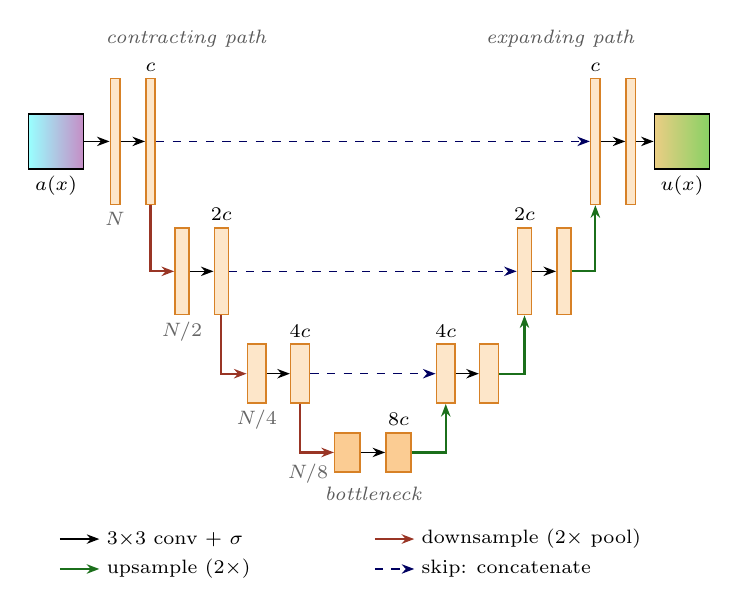
\begin{tikzpicture}[
    font=\footnotesize,
    >={Stealth[length=1.6mm]},
    every path/.style={line width=0.55pt},
    lab/.style={font=\scriptsize, inner sep=1pt},
    conv/.style={->, black},
    down/.style={->, draw=BrickRed!80!black, line width=0.8pt},
    up/.style={->, draw=ForestGreen!80!black, line width=0.8pt},
    skipc/.style={->, draw=skip, dashed},
    field/.style={draw, minimum size=0.7cm, inner sep=0pt},
  ]
  \def\yA{0}     \def\hA{1.6}  \def\wA{0.12}
  \def\yB{-1.65} \def\hB{1.1}  \def\wB{0.18}
  \def\yC{-2.95} \def\hC{0.75} \def\wC{0.24}
  \def\yD{-3.95} \def\hD{0.5}  \def\wD{0.32}

  \node[field, left color=Cyan!40, right color=Purple!45] (a) at (-0.05,\yA) {};
  \node[lab, below=1pt of a] {$a(x)$};
  \node[field, left color=Goldenrod!55, right color=OliveGreen!45] (u) at (7.9,\yA) {};
  \node[lab, below=1pt of u] {$u(x)$};

  \fmap{e0a}{0.7}{\yA}{\wA}{\hA}{local}
  \fmap{e0b}{1.15}{\yA}{\wA}{\hA}{local}
  \fmap{e1a}{1.55}{\yB}{\wB}{\hB}{local}
  \fmap{e1b}{2.05}{\yB}{\wB}{\hB}{local}
  \fmap{e2a}{2.5}{\yC}{\wC}{\hC}{local}
  \fmap{e2b}{3.05}{\yC}{\wC}{\hC}{local}
  \fmap{bna}{3.65}{\yD}{\wD}{\hD}{deep}
  \fmap{bnb}{4.3}{\yD}{\wD}{\hD}{deep}
  \fmap{d2a}{4.9}{\yC}{\wC}{\hC}{local}
  \fmap{d2b}{5.45}{\yC}{\wC}{\hC}{local}
  \fmap{d1a}{5.9}{\yB}{\wB}{\hB}{local}
  \fmap{d1b}{6.4}{\yB}{\wB}{\hB}{local}
  \fmap{d0a}{6.8}{\yA}{\wA}{\hA}{local}
  \fmap{d0b}{7.25}{\yA}{\wA}{\hA}{local}

  \foreach \p/\q in {e0a/e0b, e1a/e1b, e2a/e2b, bna/bnb, d2a/d2b, d1a/d1b, d0a/d0b}
    \draw[conv] (\p.east) -- (\q.west);
  \draw[conv] (a.east) -- (e0a.west);
  \draw[conv] (d0b.east) -- (u.west);

  \draw[down] (e0b.south) |- (e1a.west);
  \draw[down] (e1b.south) |- (e2a.west);
  \draw[down] (e2b.south) |- (bna.west);
  \draw[up]   (bnb.east) -| (d2a.south);
  \draw[up]   (d2b.east) -| (d1a.south);
  \draw[up]   (d1b.east) -| (d0a.south);

  \draw[skipc] (e0b.east) -- (d0a.west);
  \draw[skipc] (e1b.east) -- (d1a.west);
  \draw[skipc] (e2b.east) -- (d2a.west);

  \node[lab, text=black!60, anchor=north] at (0.7,-0.85) {$N$};
  \node[lab, text=black!60, anchor=north] at (1.55,-2.25) {$N/2$};
  \node[lab, text=black!60, anchor=north] at (2.5,-3.37) {$N/4$};
  \node[lab, text=black!60, anchor=north east] at (3.45,-4.05) {$N/8$};

  \node[lab, above=1pt of e0b] {$c$};
  \node[lab, above=1pt of e1b] {$2c$};
  \node[lab, above=1pt of e2b] {$4c$};
  \node[lab, above=1pt of bnb] {$8c$};
  \node[lab, above=1pt of d2a] {$4c$};
  \node[lab, above=1pt of d1a] {$2c$};
  \node[lab, above=1pt of d0a] {$c$};

  \node[lab, font=\scriptsize\itshape, text=black!65] at (1.6,1.3) {contracting path};
  \node[lab, font=\scriptsize\itshape, text=black!65] at (6.35,1.3) {expanding path};
  \node[lab, font=\scriptsize\itshape, text=black!65] at (3.975,-4.48) {bottleneck};

  \begin{scope}[shift={(0.0,-5.05)}]
    \draw[conv] (0,0) -- (0.5,0);
    \node[lab, anchor=west] at (0.55,0) {$3{\times}3$ conv + $\sigma$};
    \draw[down] (4.0,0) -- (4.5,0);
    \node[lab, anchor=west] at (4.55,0) {downsample ($2{\times}$ pool)};
    \draw[up] (0,-0.38) -- (0.5,-0.38);
    \node[lab, anchor=west] at (0.55,-0.38) {upsample ($2{\times}$)};
    \draw[skipc] (4.0,-0.38) -- (4.5,-0.38);
    \node[lab, anchor=west] at (4.55,-0.38) {skip: concatenate};
  \end{scope}
\end{tikzpicture}
\end{document}
